%\documentclass[10pt,a4paper]{article}
\documentclass[10pt,a4paper]{scrreprt}
\usepackage[utf8]{inputenc}
\usepackage{amsmath}
\usepackage{amsfonts}
\usepackage{amssymb}
\usepackage{graphicx}
\usepackage[left=2cm,right=2cm,top=2cm,bottom=2cm]{geometry}

\usepackage{tikz}
\usetikzlibrary{shapes.geometric, arrows}
\tikzstyle{io} = [trapezium, trapezium left angle=70, trapezium right angle=110, minimum width=3cm, minimum height=1cm, text centered, draw=black, fill=blue!30, text width=4cm]
\tikzstyle{process} = [rectangle, minimum width=3cm, minimum height=1cm, text centered, draw=black, fill=orange!30]
\tikzstyle{arrow} = [thick,->,>=stealth]

\usepackage{bm}
\usepackage{natbib}

% integral d
\newcommand{\myd}{\;\mathrm{d}}
% overbar
\newcommand{\overbar}[1]{\mkern 1.5mu\overline{\mkern-1.5mu#1\mkern-1.5mu}\mkern 1.5mu}

\author{Yi Hu}
\title{Homogenization for Multi Field Modelling}
\subtitle{Part I: Theories and FEniCS}


\begin{document}

\chapter{Computational Homogenization}
The method used in the current work is computational homogenization. It was proposed in 1970s by Babu\v{s}ka and collaborators \citep{EPFL-ARTICLE-184958}, while the conception of this method appeared already in the late 60s, where the one-dimensional example and examples of layered materials are already investigated \citep{cioranescu_introduction_2000}. As indicated in the name of this method, the goal is to approximate a heterogeneous problem with a homogeneous problem. The essential idea of this method is to make use of the scale separation, so that a reduced PDE for the macroscopic problem is obtained. A macroscopic problem always contains the information from its corresponding micro scale, and it is often represented as ``effective parameters''. These effective parameters are often calculated in the sense of an ``averaging procedure'' or ``homogenization''. In order to obtain homogenized quantities a micro scale problem needs to be solved. It could be solved with numerical methods such as Finite Element Method, Finite Volume Method or theoretical results in simple cases. An extensive review  can be found in \citep{efendiev2009multiscale}. A more general framework, the Heterogeneous Multiscale Method (HMM), was proposed by Bjorn Engquist. This method extend the idea of homogenization and introduce generic methodology between macro scale and micro scale. An introductory review could be found in \citep{weinan2007heterogeneous}.

The convergence of this method is given by mathematicians, which are described in detail in \citep{cioranescu_introduction_2000}. Comparison with experiments are also accomplished, which is presented in \citep{jansson_materials_1990}. Modelling examples are abundant in literatures, e.g. plasticity modelling \citep{miehe_computational_1999}, size effect and damage modelling \citep{dascalu_damage_2008}.

In this part we first illustrate the key idea of homogenization and scale separation. Then a one dimensional example is presented. Analogously we discuss the application to the 3D elliptic PDE briefly. Hill-Mandel requirements should be fulfilled in the energy conserving problem. Brief introduction of FE$^{2}$ scheme is stated in the end of this part. We confine our discussion here mainly on materials with periodic structures. 

\section{Periodic Structures}
\label{sec:peri}
Periodicity appears frequently in composite materials, for instance material with fiber or particle reinforcement. In these materials inclusions are arranged periodically. Material parameters can be expressed with periodic functions of coordinates. For example, Young's Modulus can be written in the following form,
%
\begin{equation}
\label{eq:periodic 1}
\mathbb{C}(\mathbf{x}+\mathbf{Y}) = \mathbb{C}(\mathbf{x}).
\end{equation}
%
It is often the case that discontinuity exists in composite materials. This characteristic comes from their different material properties such as Young's Modulus above. We want to represent this heterogeneous material with a homogenized one, where we have no discontinuity in material parameters and the original composite material can be treated as a homogeneous one with only one component. In addition this homogenized material should resemble the material behaviour of the heterogeneous one.

We denote $\epsilon$ as a periodicity parameter, or in other words ``the order of homogeneity". Then material parameters such as Young's modulus $\mathbb{C}$ can be written as
%
\begin{equation}
\mathbb{C}^{\epsilon}(\mathbf{x}) = \mathbb{C} \left( \dfrac{\mathbf{x}}{\epsilon} \right).
\end{equation}
%
Assumed that $\mathbb{C}$ is $\mathbf{Y}$-periodic and a reference cell of size $\mathbf{Y}$ is chosen, after transformation $\mathbb{C}^{\epsilon}$ becomes a function with period $\epsilon \mathbf{Y}$. When $\epsilon$ goes to 0, the composite material becomes more homogeneous (for a small neighbourhood the constitutes almost the same). This process is shown in the following illustration. In other words the underlying meaning of this transformation is a process of homogenization. We should notice that there are some discrepancies in the formulation of homogenization from the mathematical point of view (scale separation) and the later introduced engineering view (RVE based simulation). However the end results are the same.

\begin{figure}[h]
  \centering
    \label{fig: homo proc}
    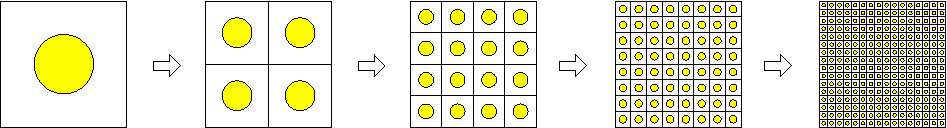
\includegraphics[width=0.8\linewidth]{../pics/homo_proc.png}
  \caption{Homogenization process with $\epsilon \to 0$}
\end{figure}

\section{Scale Separation}
When a two scale problem is addressed, a corresponding field variable could be expanded as follows, 
%
\begin{equation}
\label{eq:field epsi}
\mathbf{\Phi}^{\epsilon}(\mathbf{x}) = \mathbf{\Phi}^{0}(\mathbf{x},\mathbf{y}) + \epsilon\mathbf{\Phi}^{1}(\mathbf{x},\mathbf{y}) + \epsilon^{2} \mathbf{\Phi}^{2}(\mathbf{x},\mathbf{y}) + \cdots,
\end{equation}
%
In the above formula, $\mathbf{x}$ is the position vector of a point, which is deemed as the \textit{macroscopic} coordinate. $\mathbf{y}=\mathbf{x}/\epsilon$ is a \textit{microscopic} coordinate, which stands for \textit{rapid} oscillation. The physical nature of the right hand side is the decomposition of macro scale dependency and micro scale dependency with respect to a reference cell. The purpose of setting $\mathbf{y}=\mathbf{x}/\epsilon$ is to achieve a closed form expressed with the original coordinate. The ratio $\epsilon$ means that the micro quantity will vary $1/\epsilon$ faster than macroscopic level. When $\epsilon$ goes to $0$, functions $\mathbf{\Phi}^{0}(\mathbf{x}, \mathbf{y}), \mathbf{\Phi}^{1}(\mathbf{x}, \mathbf{y}), \cdots$ are smooth functions with respect to macroscopic coordinate and microscopic coordinate.

We should notice that functions $\mathbf{\Phi}^{i}(\mathbf{x},\mathbf{y})$ have the following properties,

\begin{equation}
\label{eq:scale separ prop}
\left\{
\begin{array}{l}
\mathbf{\Phi}^{i}(\mathbf{x},\mathbf{y}) \ \text{is defined for} \ \mathbf{x} \in \Omega \ \text{and} \ \mathbf{y} \in \mathbf{Y} \\
\mathbf{\Phi}^{i}(\cdot, \mathbf{y}) \ \text{is} \ \mathbf{Y} \text{-periodic} 
\end{array}
\right.
\end{equation}

For details we refer to chapter 6 of \citep{cioranescu_introduction_2000}. These two properties characterize the scale separation, since the first variable $\mathbf{x}$ defined in the whole domain is clearly the \textit{macroscopic} coordinate, while the second variable $\mathbf{y}$ is a coordinate in the reference cell. The setting $\mathbf{y}=\mathbf{x}/\epsilon$ describes the scale size of this problem, or the ``order of homogenization" as discussed in the previous section. If $\mathbf{Y}$ has the form $(l_{1}, \cdots, l_{N})$, then $\mathbf{x}/\epsilon = \mathbf{k}_{l} + \mathbf{y}$, where $\mathbf{k}_{l} = (k_{1}l_{1}, \cdots, k_{N}l_{N})$ and $k_{i} \in \mathbb{N}$. This shows the decomposition is valid for two scale problem and the setting $\mathbf{y}=\mathbf{x}/\epsilon$ is meaningful.

The micro-macro variable decomposition is illustrated in the following figure.

\begin{figure}[h]
  \centering
    \label{fig: scale sepa}
    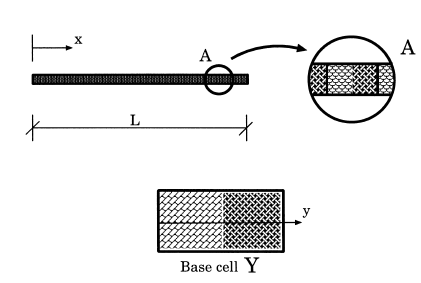
\includegraphics[width=0.45\linewidth]{../pics/ref_cell_mic_mac_coord.png}
  \caption{Micro and Macro Coordinate of Field Variable \citep{hassani1998review}}
\end{figure}

\section{One Dimensional Problem}
Many books and review papers begin with a one dimensional problem, such as \citep{cioranescu_introduction_2000}. Here we briefly go through a one dimensional elasticity problem. More detailed derivation could be found in \citep{hassani1998review}.

The governing equations, i.e. the equilibrium and Hooke's law are,
\begin{equation}
\left\{
\begin{array}{l}
\dfrac{\myd{\sigma^{\epsilon}}}{\myd{x}} + \gamma^{\epsilon} = 0 \\
\sigma^{\epsilon} = E^{\epsilon} \dfrac{\myd{u^{\epsilon}}}{\myd{x}},
\end{array}
\right.
\end{equation}

Noting that $\epsilon$ in superscript represents its periodic property. $\gamma^{\epsilon}$ is the body load of the material. If $E^{\epsilon}$ and $\gamma^{\epsilon}$ are uniform in the macro coordinate and only differ inside each cell, then the following relation holds,
\begin{equation}
E^{\epsilon}(x,x/\epsilon)=E^{\epsilon}(x/\epsilon)=E(y),
\end{equation}
The relation with respect to body load is likewise. Regarding the double scale expansion according to (\ref{eq:field epsi}) it follows with,
\begin{equation}
\label{eq:1st 1d}
\left\{
\begin{array}{l}
u^{\epsilon}(x) = u^{0}(x,y) + \epsilon u^{1}(x,y) + \epsilon^{2} u^{2}(x,y) + \cdots \\
\sigma^{\epsilon}(x) = \sigma^{0}(x,y) + \epsilon \sigma^{1}(x,y) + \epsilon^{2} \sigma^{2}(x,y) + \cdots,
\end{array}
\right.
\end{equation}

We employ the chain rule (similar for $\sigma^{i}(x, y)$), 
\begin{equation}
\label{eq:2nd 1d}
\dfrac{\myd{u^{i}(x, y)}}{\myd{x}} = \dfrac{\partial u^{i}(x, y)}{\partial x} + \dfrac{\partial u^{i}(x, y)}{\partial y} \dfrac{\myd{y}}{\myd{x}} \stackrel{y=x/\epsilon}{=} \dfrac{\partial u^{i}(x, y)}{\partial x} + \dfrac{1}{\epsilon}\dfrac{\partial u^{i}(x, y)}{\partial y}
\end{equation}

After substitution and equating the correspondent terms, we have
\begin{equation}
\label{eq: to simp 1}
\left\{
\begin{array}{l}
0 = E(y)\left( \dfrac{\partial u^{0}}{\partial y} \right) \\
\sigma^{0} = E(y) \left( \dfrac{\partial u^{0}}{\partial x} + \dfrac{\partial u^{1}}{\partial y} \right) \\
\sigma^{1} = E(y) \left( \dfrac{\partial u^{1}}{\partial x} + \dfrac{\partial u^{2}}{\partial y} \right),
\end{array}
\right.
\end{equation}
and
\begin{equation}
\label{eq: to simp 2}
\left\{
\begin{array}{l}
\dfrac{\partial \sigma^{0}}{\partial y}=0 \\
\dfrac{\partial \sigma^{0}}{\partial x} + \dfrac{\partial \sigma^{1}}{\partial y} + \gamma(y) = 0, 
\end{array}
\right.
\end{equation}
Combining the first two equations in (\ref{eq:1st 1d}) we have,
\begin{equation}
\sigma^{0} = E(y) \left( \dfrac{\partial u^{0}}{\partial x} + \dfrac{1}{\epsilon} \dfrac{\partial u^{0}}{\partial y} + \dfrac{\partial u^{1}}{\partial y} \right) =  E(y) \left( \dfrac{\myd{u^{0}}}{\myd{x}} + \dfrac{\partial u^{1}}{\partial y} \right)
\end{equation}
It follows with, 
\[
\dfrac{\sigma^{0}}{E(y)} = \dfrac{\myd{u^{0}}}{\myd{x}} + \dfrac{\partial u^{1}}{\partial y}
\]
Notice the periodicity for the second variable (\ref{eq:scale separ prop}) integration of $y$ in a reference cell yields
\begin{equation}
\label{eq: sigma 0}
\sigma^{0}(x) = \left(Y/\int_{Y} \dfrac{\myd{y}}{E(y)} \right) \dfrac{\myd{u^{0}(x)}}{\myd{x}}.
\end{equation}
Define the \textit{homogenized modulus of elasticity} as follows,
\begin{equation}
E^{H} = 1/ \left( \dfrac{1}{Y} \int_{0}^{Y} \dfrac{\myd{\eta}}{E(\eta)}\right) .
\end{equation}
Then the original problem is transformed to
\begin{equation}
\label{eq: homo 1d}
\left\{
\begin{array}{l}
\sigma^{0}(x) = E^{H} \dfrac{\myd{u^{0}(x)}}{\myd{x}} \\
\dfrac{\myd{\sigma^{0}}}{\myd{x}} + \bar{\gamma} = 0,
\end{array}
\right.
\end{equation}
where $\bar{\gamma}=1/Y \int_{Y} \gamma(y)$ is the average of $\gamma$ inside the cell, which is derived analogously using \eqref{eq: to simp 2}. From (\ref{eq: homo 1d}) the differential equation for displacement holds as
\begin{equation}
\dfrac{\myd^2 u^{0}(x)}{\myd{x^{2}}} = -\dfrac{\bar{\gamma}}{E^{H}}
\end{equation}
Taking account of the boundary condition on both ends gives the result
\[u(x) = -\dfrac{\bar{\gamma}}{E^{H}} \dfrac{x^{2}}{2} + \dfrac{\bar{\gamma}}{E^{H}} Lx \]

\section{General Elliptical PDE}
\label{sec:pde}
If a general PDE for three dimensional problem is taken into account, it would be more intricate, as the solution is often sought in the sense of weak form. In this circumstance a homogenized weak form is considered instead of the homogenized differential operator. Then the limit of homogenized weak form should converge to the weak form without homogenization, which is called \textit{G-convergence} \citep{hollister1992comparison}. As for the case of elasticity tensor in the sense of differential operator G-convergence is expressed as
\begin{equation}
\label{eq: G conv}
\lim_{\epsilon \to 0} \dfrac{\partial}{\partial x_{i}} \left[ C^{\epsilon}_{ijkl} \dfrac{\partial u^{\epsilon}_{k}}{\partial x_{l}} \right] \rightarrow \dfrac{\partial}{\partial x_{i}} \left[ \bar{C}_{ijkl} \dfrac{\partial u_{k}^{0}}{\partial x_{l}} \right]
\end{equation}
It is worth noting that when $\epsilon \to 0$, $C^{\epsilon}_{ijkl} \to C^{0}_{ijkl}$ and $u^{\epsilon}_{k} \to u^{0}_{k}$. This does not mean $u^{0}_{k}$ solves the original PDE with coefficients replaced by $C^{0}_{ijkl}$. The reason lies in that the convergence of $C_{ijkl}$ and $u_{k}$ is weakly convergent. In this context, the limit of product does not equal to the product of the convergent limits. We should specify a new $\bar{C}_{ijkl}$, which gives the result $u^{0}$. Thorough discussion on this point can be found in \citep{cioranescu_introduction_2000}. A quick overview of the general problem is given in the review \citep{hassani1998review}. Several key points of the general problem are listed here. With the notation of general elliptical operator using 
\begin{equation}
\mathcal{A}^{\epsilon} = \dfrac{\partial}{\partial x_{i}} \left( a_{ij}(\mathbf{y}) \dfrac{\partial}{\partial x_{j}} \right).
\end{equation}
general problem could then be described as,
\begin{equation}
\left\{
\begin{array}{ll}
\mathcal{A}^{\epsilon} \mathbf{u^{\epsilon}}= \mathbf{f} & \text{in} \ \Omega \\
\mathbf{u}^{\epsilon} = \mathbf{0} & \text{on} \ \partial \Omega
\end{array}
\right.
\end{equation}
Employing the double scale expansion for both the field variable $\mathbf{u}^{\epsilon}$ and the differential operator $\mathcal{A}^{\epsilon}$, namely (notice that chain rule is applied when differentiating)
\begin{equation}
\left\{
\begin{array}{l}
\mathbf{u}^{\epsilon}(\mathbf{x}) = \mathbf{u}^{0}(\mathbf{x},\mathbf{y}) + \epsilon \mathbf{u}^{1}(\mathbf{x},\mathbf{y}) + \epsilon^{2} \mathbf{u}^{2}(\mathbf{x},\mathbf{y}) + \cdots \\
\mathcal{A}^{\epsilon} = \dfrac{1}{\epsilon^{2}} \mathcal{A}^{1} + \dfrac{1}{\epsilon} \mathcal{A}^{2} + \mathcal{A}^{3}
\end{array}
\right.
\end{equation}
Here $\mathcal{A}^{1}, \mathcal{A}^{2}, \mathcal{A}^{3}$ is defined as follows
\[
\mathcal{A}^{1} = \dfrac{\partial}{\partial y_{i}} \left( a_{ij}(\mathbf{y}) \dfrac{\partial}{\partial y_{j}} \right); \
\mathcal{A}^{2} = \dfrac{\partial}{\partial y_{i}} \left( a_{ij}(\mathbf{y}) \dfrac{\partial}{\partial x_{j}} \right) + \dfrac{\partial}{\partial y_{i}} \left( a_{ij}(\mathbf{y}) \dfrac{\partial}{\partial x_{j}} \right); \
\mathcal{A}^{3} = \dfrac{\partial}{\partial x_{i}} \left( a_{ij}(\mathbf{y}) \dfrac{\partial}{\partial x_{j}} \right).
\]
Substitution with the above differential operators and comparing with the according terms give
\begin{equation}
\label{eq: eq group}
\left\{
\begin{array}{l}
\mathcal{A}^{1} \mathbf{u}^{0} = \mathbf{0} \\
\mathcal{A}^{1} \mathbf{u}^{1} + \mathcal{A}^{2} \mathbf{u}^{0} = \mathbf{0} \\
\mathcal{A}^{1} \mathbf{u}^{2} + \mathcal{A}^{2} \mathbf{u}^{1} + \mathcal{A}^{3} \mathbf{u}^{0} = \mathbf{f}.
\end{array}
\right.
\end{equation}
From \citep{cioranescu_introduction_2000} it is known that if a $\mathbf{Y}$-periodic function $u$ has a unique solution in terms of $\mathcal{A}^{1}$ operator, i.e. 
\begin{equation}
\mathcal{A}^{1} \mathbf{u} = \mathbf{F} \quad \text{in reference cell}.
\end{equation}
Then the right hand side of the above equation, $\mathbf{F}$ should satisfy 
\begin{equation}
\overbar{\mathbf{F}} = \dfrac{1}{|Y|}\int_{Y} \mathbf{F} \myd{\mathbf{y}} = \mathbf{0}.
\end{equation}
Applying this proposition to (\ref{eq: eq group}) several times the field variable could be expressed with the following form,
\begin{equation}
\mathbf{u}^{1}(\mathbf{x}, \mathbf{y}) = \chi^{i}(\mathbf{y}) \dfrac{\partial \mathbf{u}(\mathbf{x})}{\partial x_{j}} + \mathbf{\xi} (\mathbf{x})
\end{equation}
Function $\chi^{i}(\mathbf{y})$ is the local solution of this problem, which has $\mathbf{Y}$-periodic property. And $\xi(\mathbf{x})$ is the solution of macro scale. The local problem is
\begin{equation}
\mathcal{A}^{1} \mathbf{\chi}^{j}(\mathbf{y}) = \dfrac{\partial a_{ij}(\mathbf{y})}{\partial y_{i}} \quad \text{in reference cell}.
\end{equation}
Hence the macro scale problem (homogenized problem) can be written as
\begin{equation}
\mathcal{A}^{H} \mathbf{u} = \mathbf{f},
\end{equation}
with
\begin{equation}
\mathcal{A}^{H} = a^{H}_{ij} \dfrac{\partial^{2}}{\partial x_{i} \partial x_{j}}.
\end{equation}
%
And the effective coefficients are related with the solution of micro scale problem, i.e.
\begin{equation}
a^{H}_{ij} = \dfrac{1}{|Y|} \int_{Y} \left( a_{ij}(\mathbf{y}) + a_{ik}(\mathbf{y}) \dfrac{\partial \chi^{j}}{\partial y_{k}} \right) \myd{\mathbf{y}}
\end{equation}

%--------------------------------
\section{Hill-Mandel Condition}
After introducing the general mathematical concepts about homogenization methods, we move to its application in material modelling. From the perspective of material modelling a Representative Volume Element (RVE) is investigated. This concept coincides with \textit{reference cell} in the previous section from the mathematical perspective. In such an RVE, size is not what we are concerned with, since the homogenization will lead to $\epsilon \to 0$, meaning the size of RVE going against 0, achieving a homogeneous state. This homogenization process and the underlying reason was elaborated in the previous section \ref{sec:peri}. Hence such RVE is often take as a unit cell, other geometry configurations are explored in \citep{gluge2012comparison}. 

In homogenization of an RVE the key step is to obtain coefficients for the macro scale PDE. For material modelling such coefficients are material parameters, i.e. tangent moduli. The behaviour of RVE should resemble the material in this scale. Therefore the model for micro scale should be able to capture specific features, where the continuum mechanical equilibrium of composites in the micro scale is always established. Such equilibrium can be formulated in various ways. The method utilized in this student project is an energy based description. The connection between micro and macro scale is called Hill-Mandel condition \citep{hill_essential_1967}. In a recent paper the relation of Irving-Kirkwood theory and Hill-Mandel homogenization theory is revealed \citep{mercer_novel_2015}.

The Hill-Mandel condition states that the total stress power on the micro scale should be equal to the stress power at relevant point on the macro scale. For small strain, the following equation holds,

\begin{equation}
\left< \bm{\sigma} \cdot \dot{\bm{\varepsilon}} \right> = \left< \bm{\sigma} \right> \cdot \left< \dot{\bm{\varepsilon}} \right>,
\end{equation}
where $\left< \cdot \right>$ means averaging of the considered variable. In simulations certain boundary conditions are devised to fulfil Hill-Mandel condition automatically. 

To solve PDEs for the micro state various issues arise. To input the information from the macro scale, averaged field variable from the macro scale was inserted in the formulation. The boundary condition of micro scale model should also be compatible within the context of homogenization. Various function spaces are devised to fulfil this point. The most common three boundary conditions for RVE simulations are Linear Displacement Boundary Condition (LDBC), Homogeneous Traction Boundary Condition (HTBC), and Periodic Boundary Condition (PBC) \citep{gluge2012comparison}. It can be shown that function spaces with these three common boundary conditions satisfy Hill-Mandel condition a priori. For simulations of other kinds such as thermo-mechanical or porous medium, we refer to \citep{mandadapu_homogenization_2012}, \citep{ozdemir_computational_2008}, and \citep{gray_solid_2009}.

The formulation of Hill-Mandel condition in implementation aspects can be referred in \citep{miehe_computational_2002}, where Lagrangian Multiplier is used to enforce Hill-Mandel condition.

%\bibliographystyle{plain}
%\bibliography{/home/yihu/studien_arbeit_fenics/report/part1/part1_ref.bib}
%\nocite{*}

\section{Basic Concepts of FE$^{2}$ Scheme}
Embedding a micro scale computation on an RVE into a macro scale computation is the essential idea of FE$^{2}$ scheme. Related works concerning micro-macro coupling can be found in \citep{miehe_computational_1999-1} \citep{miehe_computational_2002} \citep{miehe_computational_2003} \citep{miehe_strain-driven_2002} \citep{miehe_homogenization_2002}. Here we present the idea from \citep{miehe_computational_1999-1}, which is the basics of FE$^{2}$ scheme. Although in a different notation, the following formulation can be well compared with the one presented in section \ref{sec:pde}.

For large strain problem the macro scale problem is, 
\begin{equation}
\label{eq:macro}
\left\{
\begin{array}{ll}
\textrm{Div} \; \overbar{\mathbf{P}} + \overbar{\mathbf{\gamma}} = \mathbf{0} & \text{in} \ \mathcal{B} \\
\overbar{\mathbf{t}} = \overbar{\mathbf{t}}_{b} & \text{on} \ \partial \mathcal{B}_{f} 
\\
\overbar{\mathbf{x}} = \overbar{\mathbf{x}}_{b} & \text{on} \ \partial \mathcal{B}_{x} 
\end{array}
\right.
\end{equation}
At the same time we have micro scale problem as follows
\begin{equation}
\label{eq:micro}
\left\{
\begin{array}{ll}
\textrm{Div} \; \mathbf{P} = \mathbf{0} & \text{in} \ \mathcal{RVE} \\
\widetilde{\mathbf{w}}^{+} = \widetilde{\mathbf{w}}^{-} & \text{on} \ \partial \mathcal{RVE} 
\end{array}
\right.
\end{equation}
where $\overbar{(\cdot)}$ stands for macro field averages, and $\widetilde{(\cdot)}$ represents micro field fluctuations. $(\cdot)^{+}$ and $(\cdot)^{-}$ are the corresponding fluctuation pair on the boundary. The relation between micro scale and macro scale is 
\begin{equation}
\mathbf{x} = \overbar{\mathbf{F}} \mathbf{X} + \widetilde{\mathbf{w}} \ \text{in} \ \mathcal{RVE}
\end{equation}

The effective tangent moduli is derived from the averaged stress and strain,
\begin{equation}
\label{eq:avg}
\overbar{\mathbf{P}} = \dfrac{1}{V} \int_{\mathcal{RVE}} \mathbf{P} \myd{\mathbf{x}}, \quad 
\overbar{\mathbf{F}} = \dfrac{1}{V} \int_{\mathcal{RVE}} \mathbf{F} \myd{\mathbf{x}}
\end{equation}
\begin{equation}
\label{eq:mima}
\Delta \overbar{\mathbf{P}} = \mathbb{C}_{\text{eff}} \Delta \overbar{\mathbf{F}} 
\end{equation}

The weak form of micro scale problem is 
\begin{equation}
\label{eq:wf}
G = \int_{\mathcal{RVE}} \delta \widetilde{\mathbf{F}} : \mathbf{P} \myd{\mathbf{x}}.
\end{equation}
The linearization of the above weak form can be written as 
\begin{equation}
\label{eq:lin}
G + \Delta G = G + \int_{\mathcal{RVE}} \delta \widetilde{\mathbf{F}} : \mathbb{C} : \left( \Delta \overbar{\mathbf{F}} + \Delta \widetilde{\mathbf{F}} \right) \myd{\mathbf{x}}
\end{equation}
Noting $\widetilde{\mathbf{F}} = \nabla{\widetilde{\mathbf{w}}}$ and taking both \eqref{eq:wf} and \eqref{eq:lin} zero it follows with

\begin{equation}
\label{eq:interm}
\int_{\mathcal{RVE}} \delta \nabla{\widetilde{\mathbf{w}}} : \mathbb{C} : \left( \Delta \overbar{\mathbf{F}} + \Delta \nabla{\widetilde{\mathbf{w}}} \right) \myd{\mathbf{x}} = 0
\end{equation}

After discretization using $\widetilde{\mathbf{w}}^{h} = \mathbf{N} \mathbf{d}$, $\nabla \widetilde{\mathbf{w}}^{h} = \mathbf{B} \mathbf{d}$, and $\mathbb{C} : \nabla \widetilde{\mathbf{w}}^{h} = \mathbf{L} \mathbf{d}$. The corresponding stiffness matrix is denoted as $\mathbf{K}$. Then \eqref{eq:interm} is simplified as 
\begin{equation}
\mathbf{K} \Delta \widetilde{\mathbf{d}} = - \mathbf{L} \Delta \overbar{\mathbf{F}}
\end{equation}

Inserting this relation into averaged stress \eqref{eq:avg} gives
\begin{equation}
\begin{split}
\overbar{\mathbf{P}} & = \dfrac{1}{V} \int_{\mathcal{RVE}} \mathbf{P} \myd{\mathbf{x}} \\ & = \dfrac{1}{V} \int_{\mathcal{RVE}} \mathbb{C} : \left( \Delta \overbar{\mathbf{F}} + \Delta \nabla{\widetilde{\mathbf{w}}^{h}} \right) \myd{\mathbf{x}} \\
& = \dfrac{1}{V} \int_{\mathcal{RVE}} \mathbb{C} : \Delta \overbar{\mathbf{F}} \myd{\mathbf{x}} + \dfrac{1}{V} \mathbf{L}^{T} \Delta \widetilde{\mathbf{d}} \Delta \overbar{\mathbf{F}}\\
& = \dfrac{1}{V} \int_{\mathcal{RVE}} \mathbb{C} : \Delta \overbar{\mathbf{F}} \myd{\mathbf{x}} - \dfrac{1}{V} \mathbf{L}^{T} \mathbf{K}^{-1} \mathbf{L} \Delta \overbar{\mathbf{F}} 
\end{split}
\end{equation}
This expression gives the end result of the effective tangent moduli
\begin{equation}
\label{eq:eff tan}
\mathbb{C}_{\text{eff}} = \dfrac{1}{V} \int_{\mathcal{RVE}} \mathbb{C} \myd{\mathbf{x}} - \dfrac{1}{V} \mathbf{L}^{T} \mathbf{K}^{-1} \mathbf{L} 
\end{equation}
\eqref{eq:macro}, \eqref{eq:mima}, and \eqref{eq:eff tan} constitute the governing equation of macro scale, which is to be solved in the sense of common FE formulation. 

To sum up in the complete FE$^{2}$ scheme micro computation and macro computation runs alternatively. When the deformation from the macro scale problem is obtained through \eqref{eq:macro}, one can start to solve the micro scale problem with the averaged strain calculated from the macro scale. After solving the fluctuation of the micro scale problem, the current averaged tangent moduli can be determined. In the meanwhile the second term of the effective tangent moduli can be evaluated. Combining the above two leads to a full representation effective tangent moduli, which is plugged into the macro scale problem. Then the solving of a macro scale problem will start again. This is illustrated in the following diagram.

\begin{figure}[h]
\centering
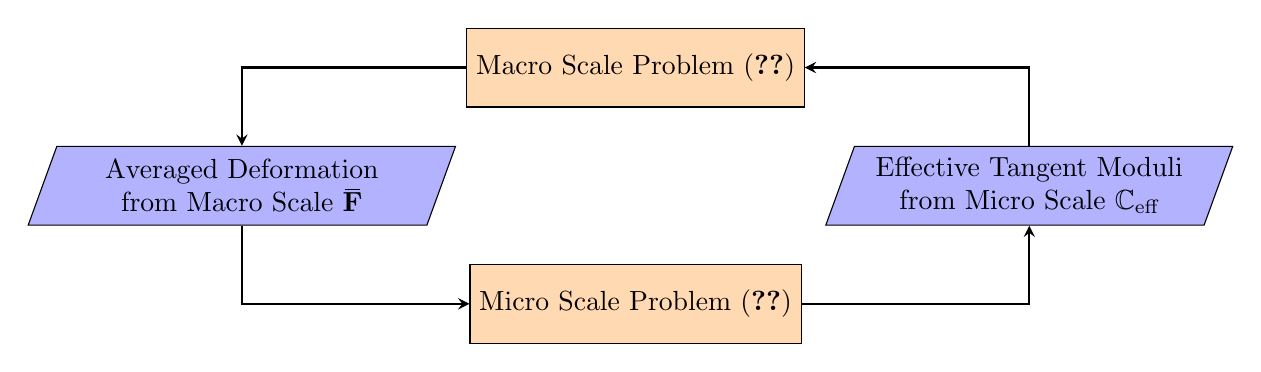
\begin{tikzpicture}[node distance=3cm]

\node (ma) [process] {Macro Scale Problem \eqref{eq:macro}};
\node (mi) [process, below of=ma] {Micro Scale Problem \eqref{eq:micro}};
\node (F) [io, left of=ma, xshift = -2cm, yshift=-1.5cm] {Averaged Deformation from Macro Scale $\overbar{\mathbf{F}}$};
\node (C) [io, left of=ma, xshift = +8cm, yshift=-1.5cm] {Effective Tangent Moduli from Micro Scale $\mathbb{C}_{\text{eff}}$};

\draw [arrow] (ma) -| (F);
\draw [arrow] (F) |- (mi);
\draw [arrow] (mi) -| (C);
\draw [arrow] (C) |- (ma);
\end{tikzpicture}
\caption{FE$^{2}$ Scheme}
\end{figure}

This scheme is extended for multiple fields in the second part of report.

\end{document}



